\noindent {\bf You may want to run one case with the same parameters as in your code from Problem Set \#3 and include in the report, to verify to me as well as yourself that you obtain the same results.}\\

To verify the correctness of the code, we compute a subsonic case to compare with the pre-existing MATLAB code. We compute the flow about a NACA 0010 airfoil (TH = 0.10) for $M_\infty = 0.0$ (incompressible) without wind tunnel wall (iwall = 0) and with a default grid of:

\begin{center}
\begin{tabular}{@{} l l l l @{}}
    JLE = 33  & JTE = 63  & JMAX = 95  & KMAX = 33 \\
    DXDY = 1  & XSF = 1.18  & YSF = 1.18  & KCONST = 3
\end{tabular}    
\end{center}

Plotting the pressure distribution along the airfoil surface, we obtain the plot shown in Figure \ref{fig:pressure_coefficient-1}. For comparison, the same plot is shown in Figure \ref{fig:pressure_coefficient-1} generated from the MATLAB code.  We can see from the plots, that the pressure distribution is the same and the number of iterations required to reduce the $L_2$ norm of the residual by approximately three orders of magnitude is also the same. Furthermore, we can see that the pressure distribution in both cases follows the Prandtl-Glauert correction to data from Abbot and von Doenhoff for linearized compressible flow. This shows that the Python code is working correctly.

\begin{figure}
    \centering
    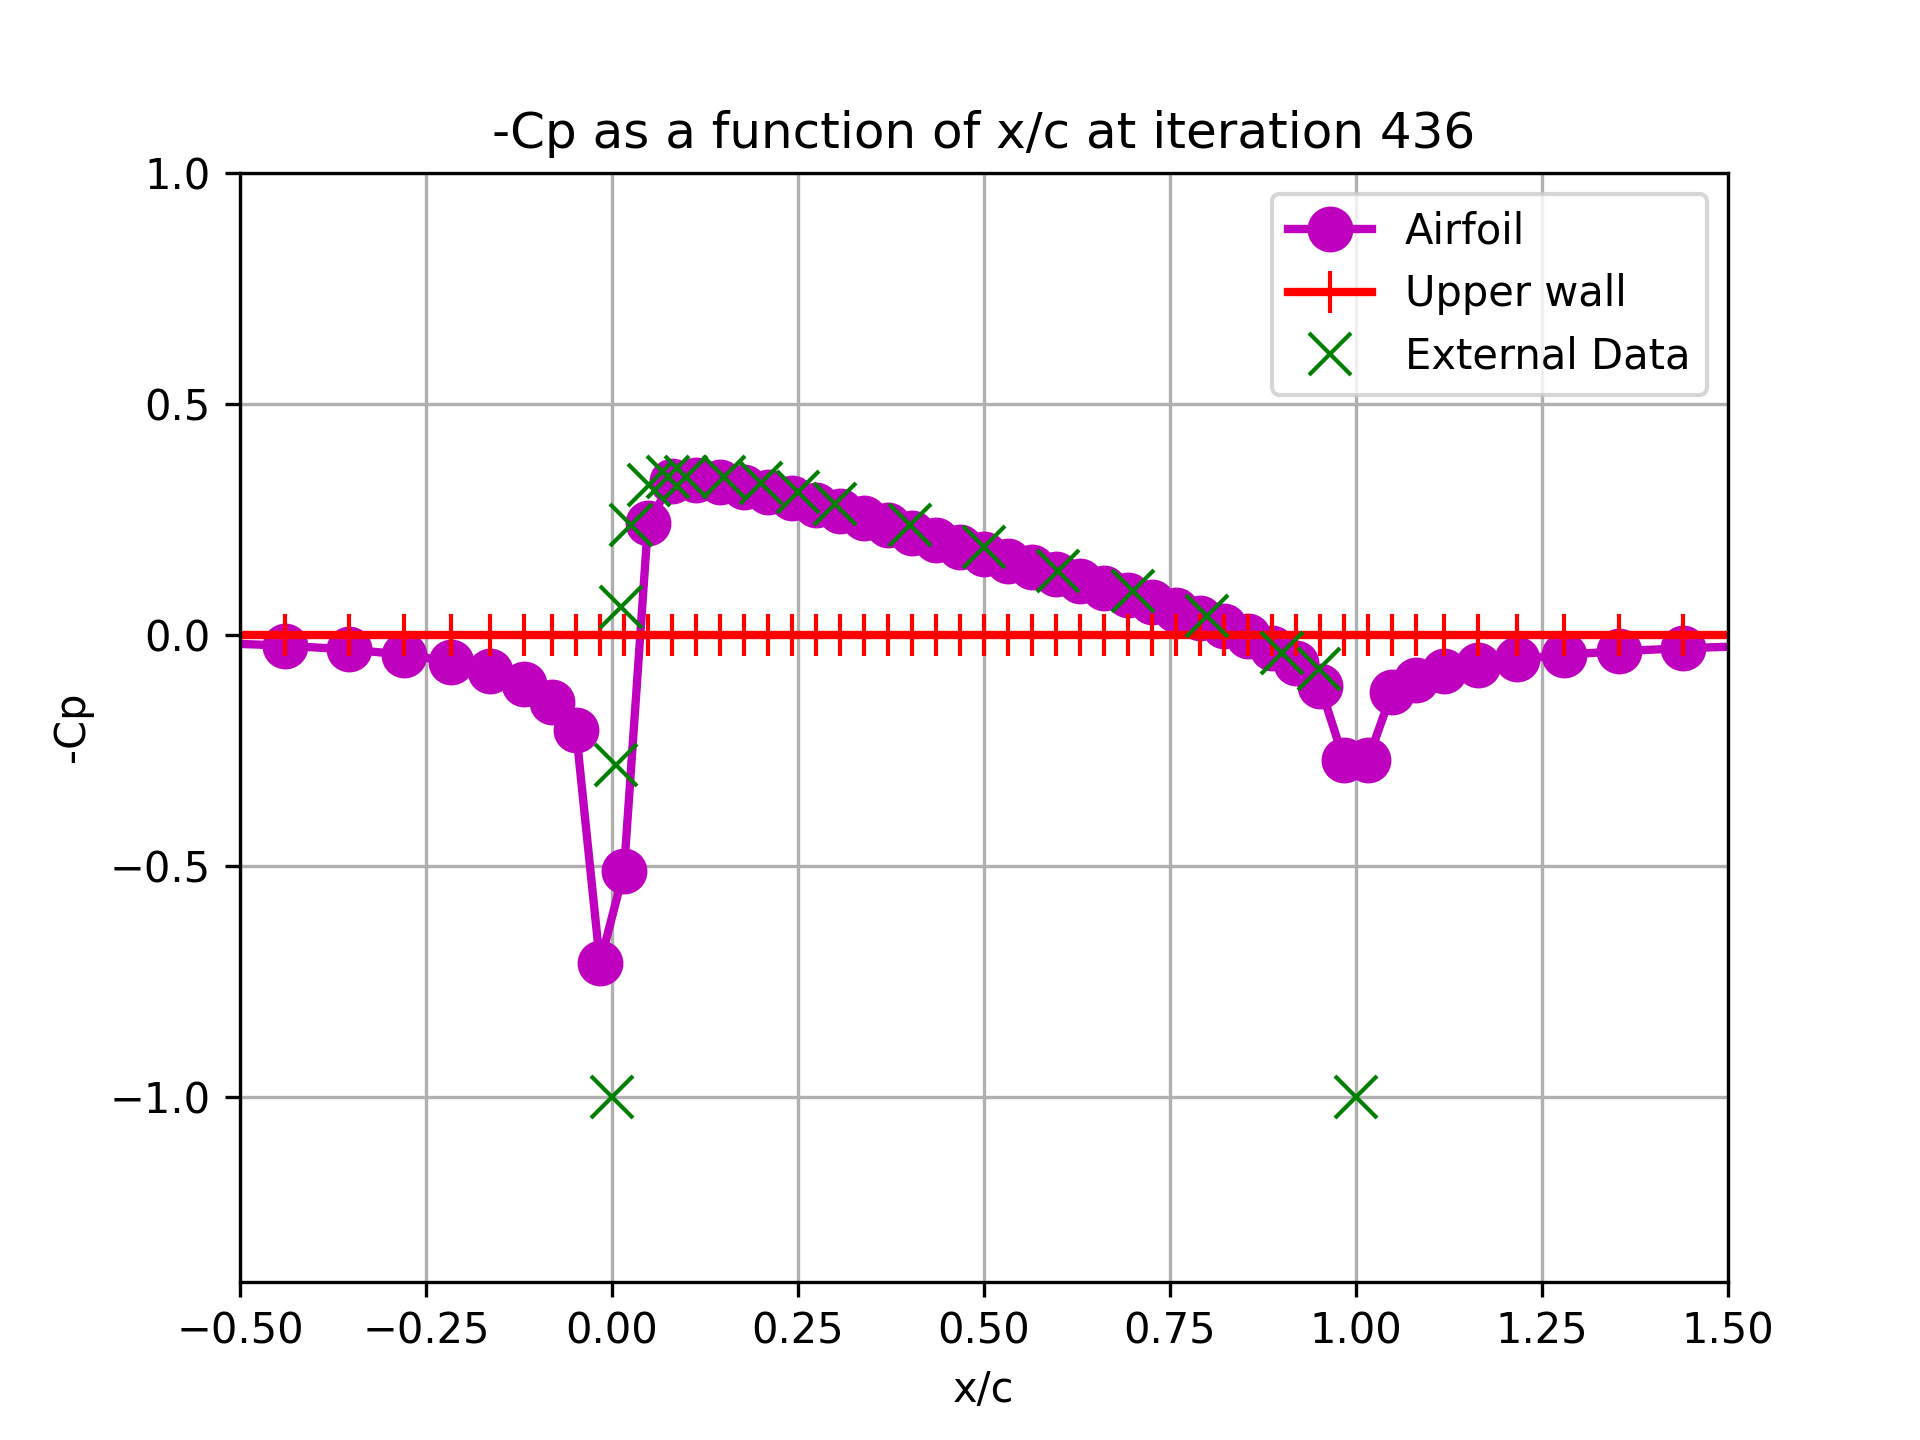
\includegraphics[width=0.75\textwidth,height=\textwidth,keepaspectratio]{images/pressure_coefficient-1.png}
    \caption{Pressure distribution along the airfoil surface for NACA 0010 airfoil at $M_\infty = 0.0$ using Python code.}
    \label{fig:pressure_coefficient-1}
\end{figure}

\begin{figure}
    \centering
    \includegraphics[width=0.75\textwidth,height=\textwidth,keepaspectratio]{images/pressure_coefficient-0.png}
    \caption{Pressure distribution along the airfoil surface for NACA 0010 airfoil at $M_\infty = 0.0$ using MATLAB code.}
    \label{fig:pressure_coefficient-0}
\end{figure}

\vspace{1cm}


\noindent {\bf Include a table showing the different cases run, the number of iterations required for convergence, number of supersonic points, total CPU time, etc.}\\

We continue to run the code for a NACA 0010 airfoil and a biconvex airfoil (TH = 0.10) for $M_\infty = 0.75$ and $M_\infty = 0.8$ in air ($\gamma = 1.4$) respectively. These computations are done with a default grid of

\begin{center}
    \begin{tabular}{@{} l l l l @{}}
        JLE = 33  & JTE = 73  & JMAX = 105  & KMAX = 43 \\
        DXDY = 1  & XSF = 1.2  & YSF = 1.2  & KCONST = 3
    \end{tabular}    
\end{center}


We also preform two additional cases, first a NACA 0010 airfoil at $M_\infty = 0.75$ with the wind tunnel one chord above the centerline (with equal spacing in the y-direction) and secondly a NACA 0010 airfoil at $M_\infty = 0.80$ using a fine grid of

\begin{center}
    \begin{tabular}{@{} l l l l @{}}
        JLE = 63  & JTE = 123  & JMAX = 185  & KMAX = 63 \\
        DXDY = 1  & XSF = 1.1  & YSF = 1.0  & KCONST = 3
    \end{tabular}    
\end{center}

All cases were run until either the number of iterations exceeded 1000 or the $L_2$ norm of the residual was reduced by three orders of magnitude. The number of iterations required, the number of supersonic points at the final iteration, and the total CPU time are summarized in Table \ref{tab:results}. From now on, we will refer to each set of parameters using the case number presented in \ref{tab:results}.

\begin{table}[h]
    \centering
    \begin{tabular}{c l c c c c c c}
        \hline
        Case & Airfoil & $M_\infty$ & Grid Type & Wind Tunnel & Iterations & Supersonic Points & CPU Time (s) \\
        \hline
        1 & NACA 0010 & 0.75 & Default & None & 1000 & 0 & 19.9 \\
        2 & Biconvex & 0.75 & Default & None & 601 & 0 & 12.1 \\
        3 & NACA 0010 & 0.80 & Default & None & 1000 & 10 & 20.1 \\
        4 & Biconvex & 0.80 & Default & None & 1000 & 21 & 19.9 \\
        5 & NACA 0010 & 0.75 & Default & Yes & 1000 & 1 & 20.19 \\
        6 & NACA 0010 & 0.80 & Stretched & None & 1000 & 18 & 52.9 \\
        \hline
    \end{tabular}
    \caption{Summary of computations: number of iterations, supersonic points, and CPU time.}
    \label{tab:results}
\end{table}

\vspace{1cm}



\noindent {\bf Include figures that show the pressure distribution on the airfoil by plotting the pressure coefficient versus x/c along the airfoil.}\\

We can plot the pressure distribution on the airfoil $-C_p$ and compare it to $x/c$ along the airfoil. The results for cases 1-6 are shown in Figures \ref{fig:pressure_coefficient-2} - \ref{fig:pressure_coefficient-7} respectively.

\begin{figure}
    \centering
    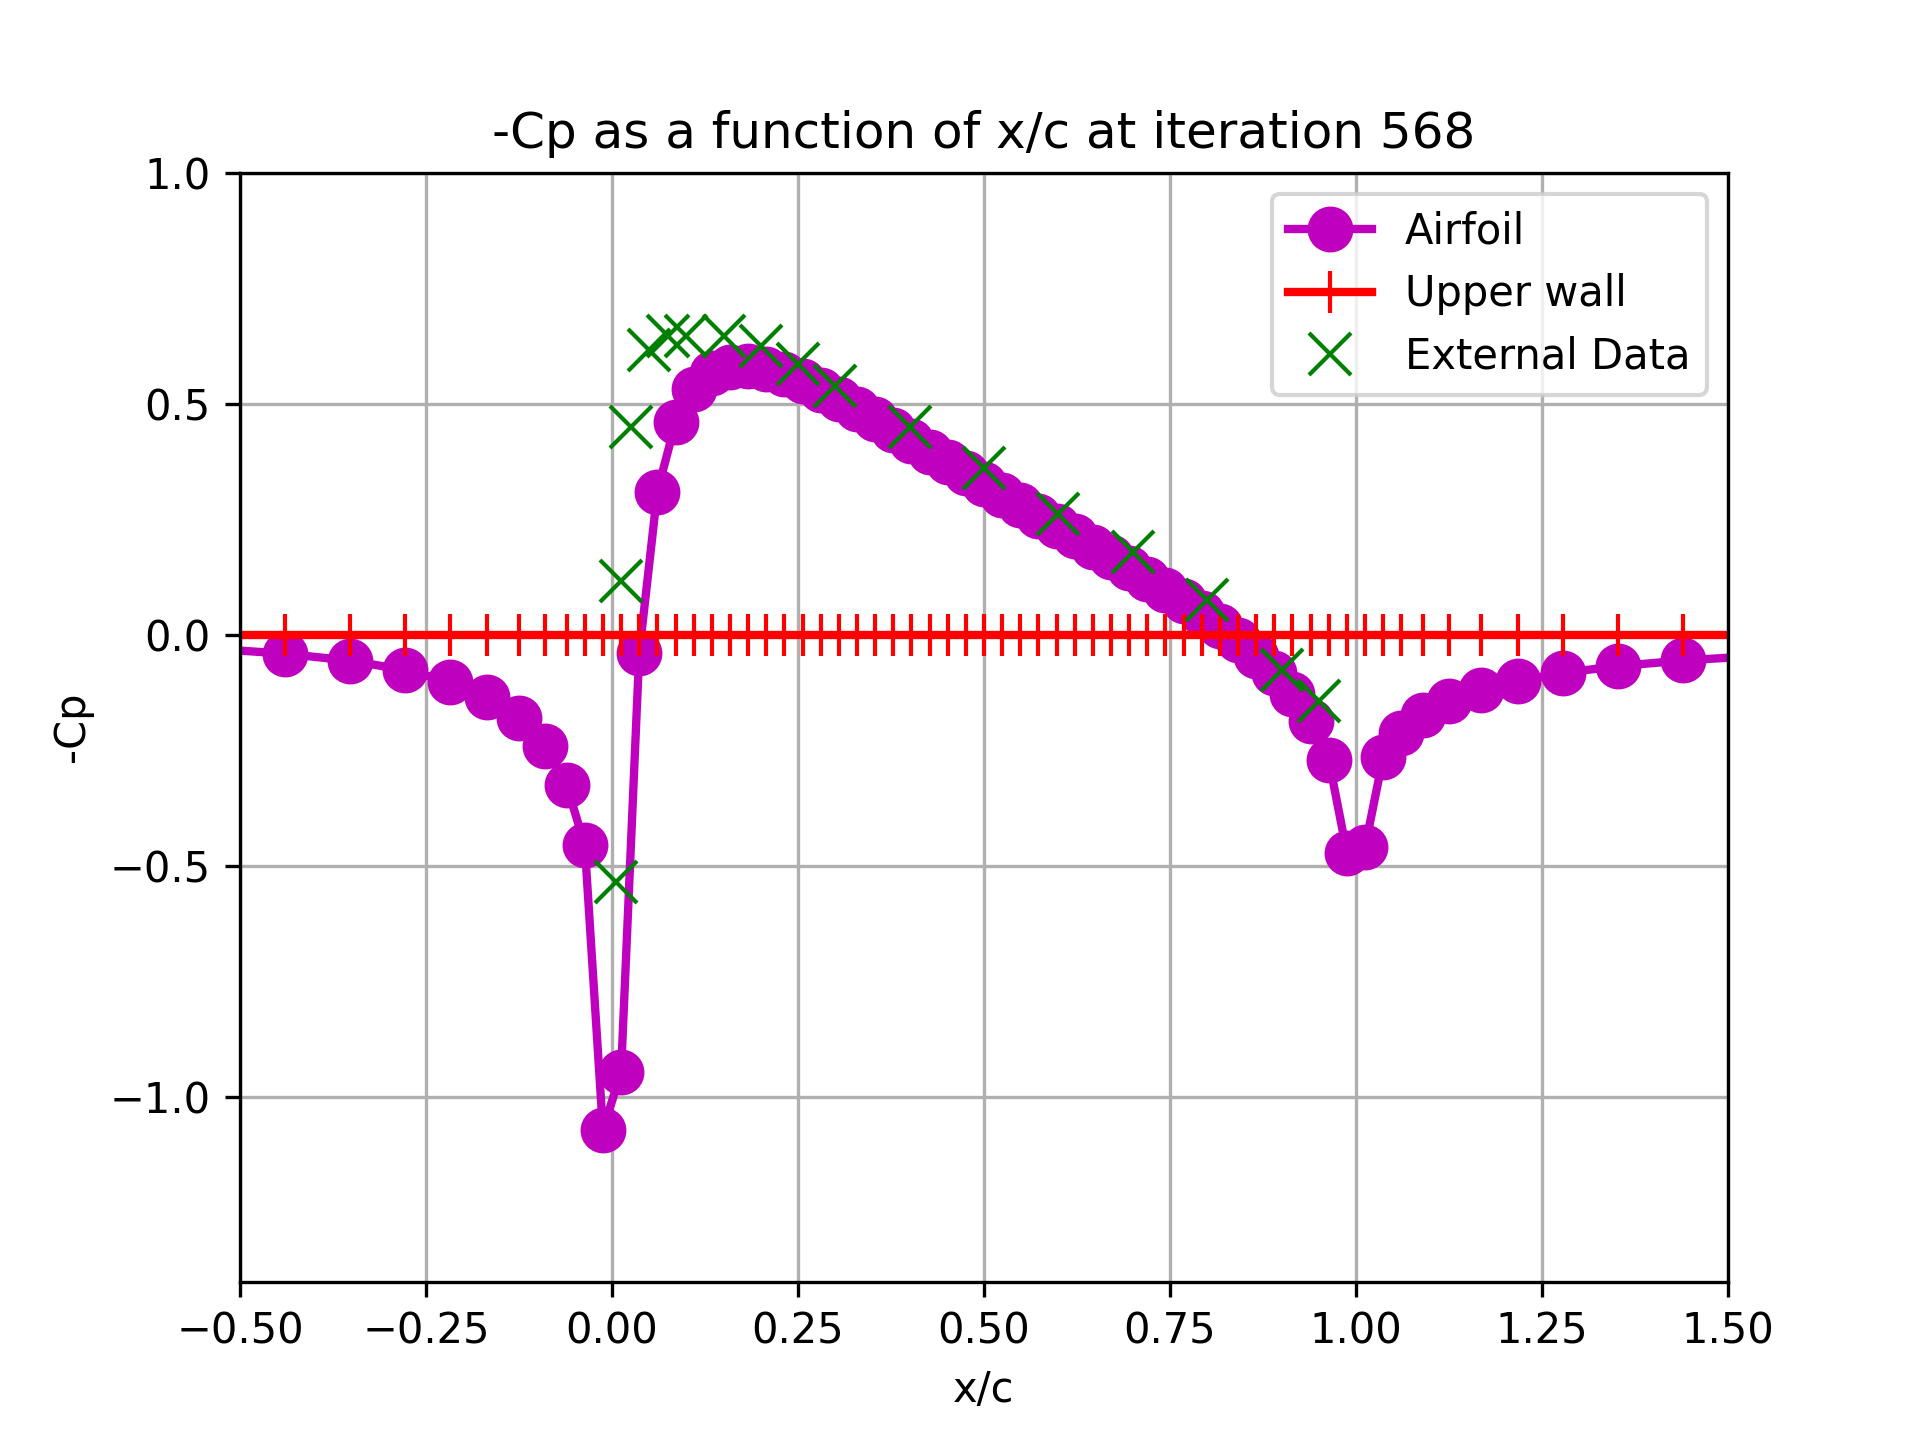
\includegraphics[width=0.75\textwidth,height=\textwidth,keepaspectratio]{images/pressure_coefficient-2.png}
    \caption{Pressure distribution $-C_p$ compared to $x/c$ along the airfoil surface for NACA 0010 airfoil at $M_\infty = 0.75$.}
    \label{fig:pressure_coefficient-2}
\end{figure}

\begin{figure}
    \centering
    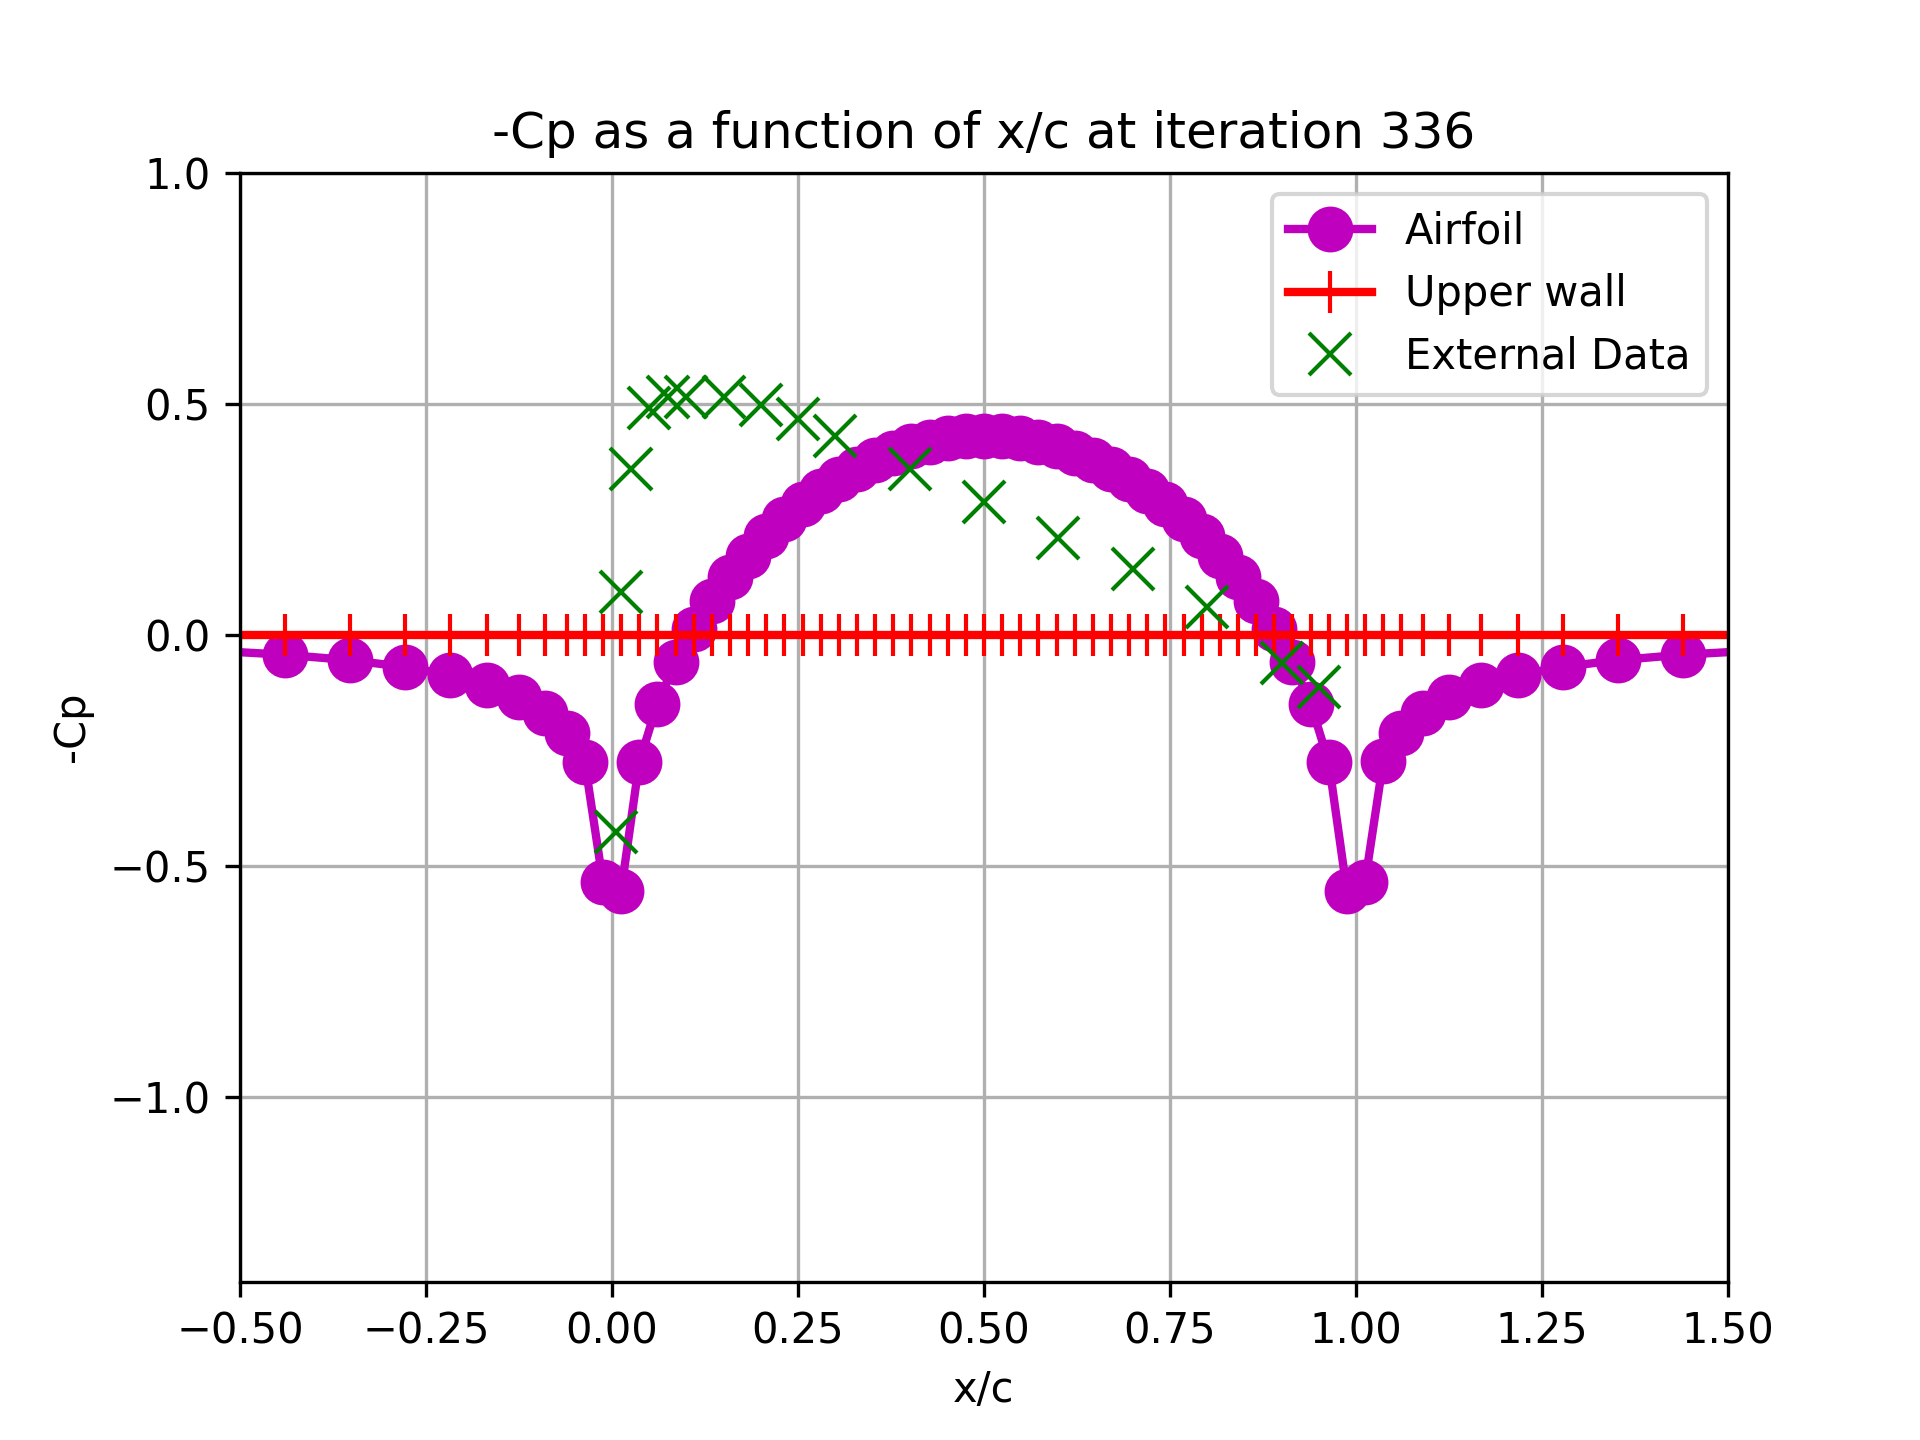
\includegraphics[width=0.75\textwidth,height=\textwidth,keepaspectratio]{images/pressure_coefficient-3.png}
    \caption{Pressure distribution $-C_p$ compared to $x/c$ along the airfoil surface for Biconvex 0010 airfoil at $M_\infty = 0.75$.}
    \label{fig:pressure_coefficient-3}
\end{figure}

\begin{figure}
    \centering
    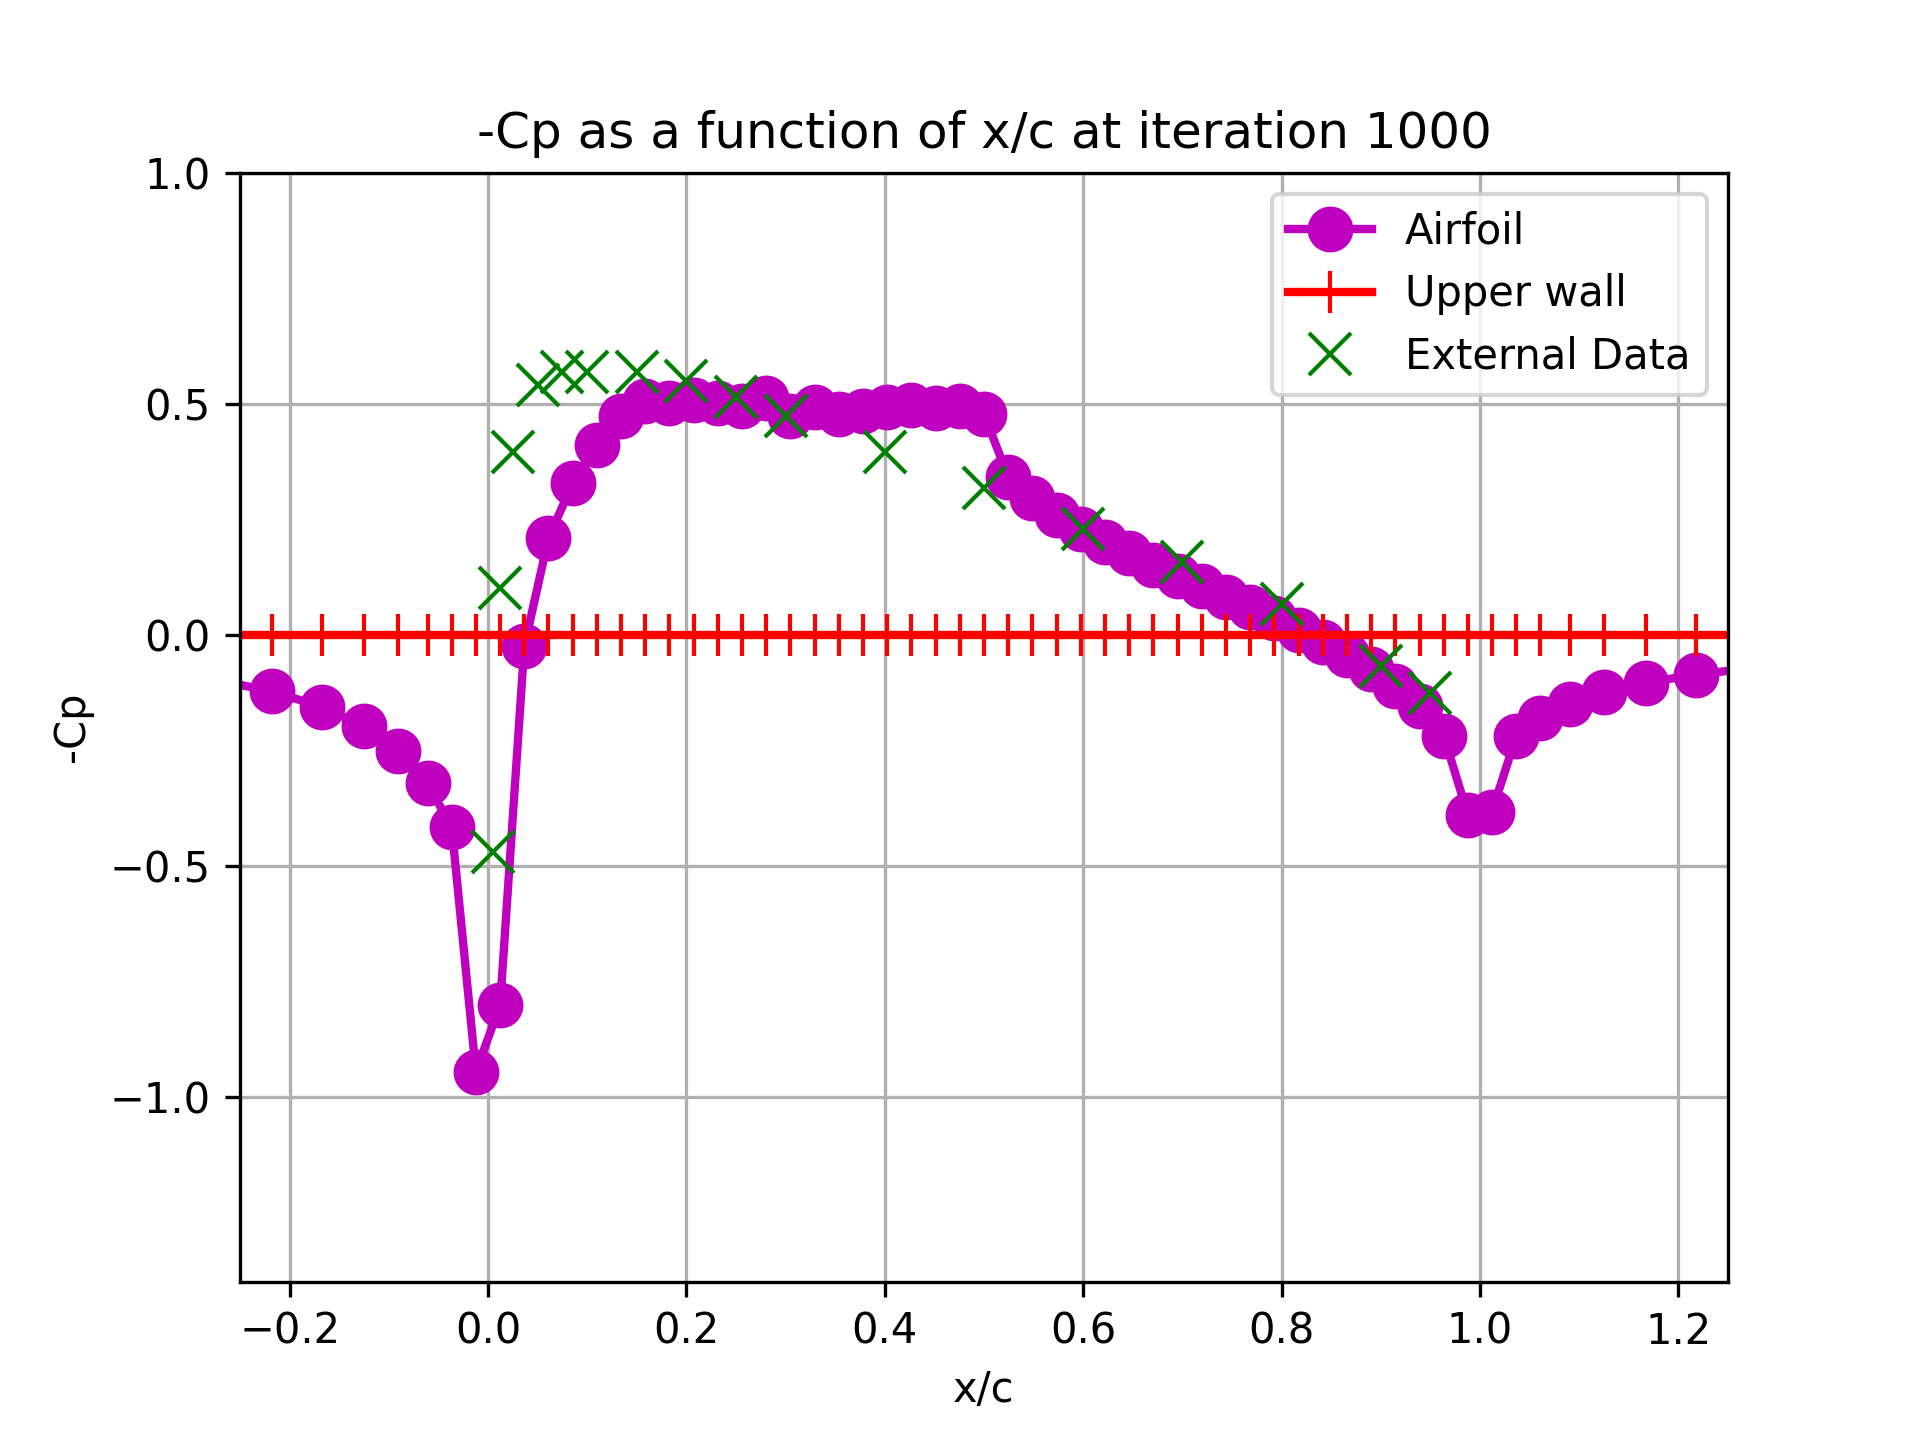
\includegraphics[width=0.75\textwidth,height=\textwidth,keepaspectratio]{images/pressure_coefficient-4.png}
    \caption{Pressure distribution $-C_p$ compared to $x/c$ along the airfoil surface for NACA 0010 airfoil at $M_\infty = 0.80$.}
    \label{fig:pressure_coefficient-4}
\end{figure}

\begin{figure}
    \centering
    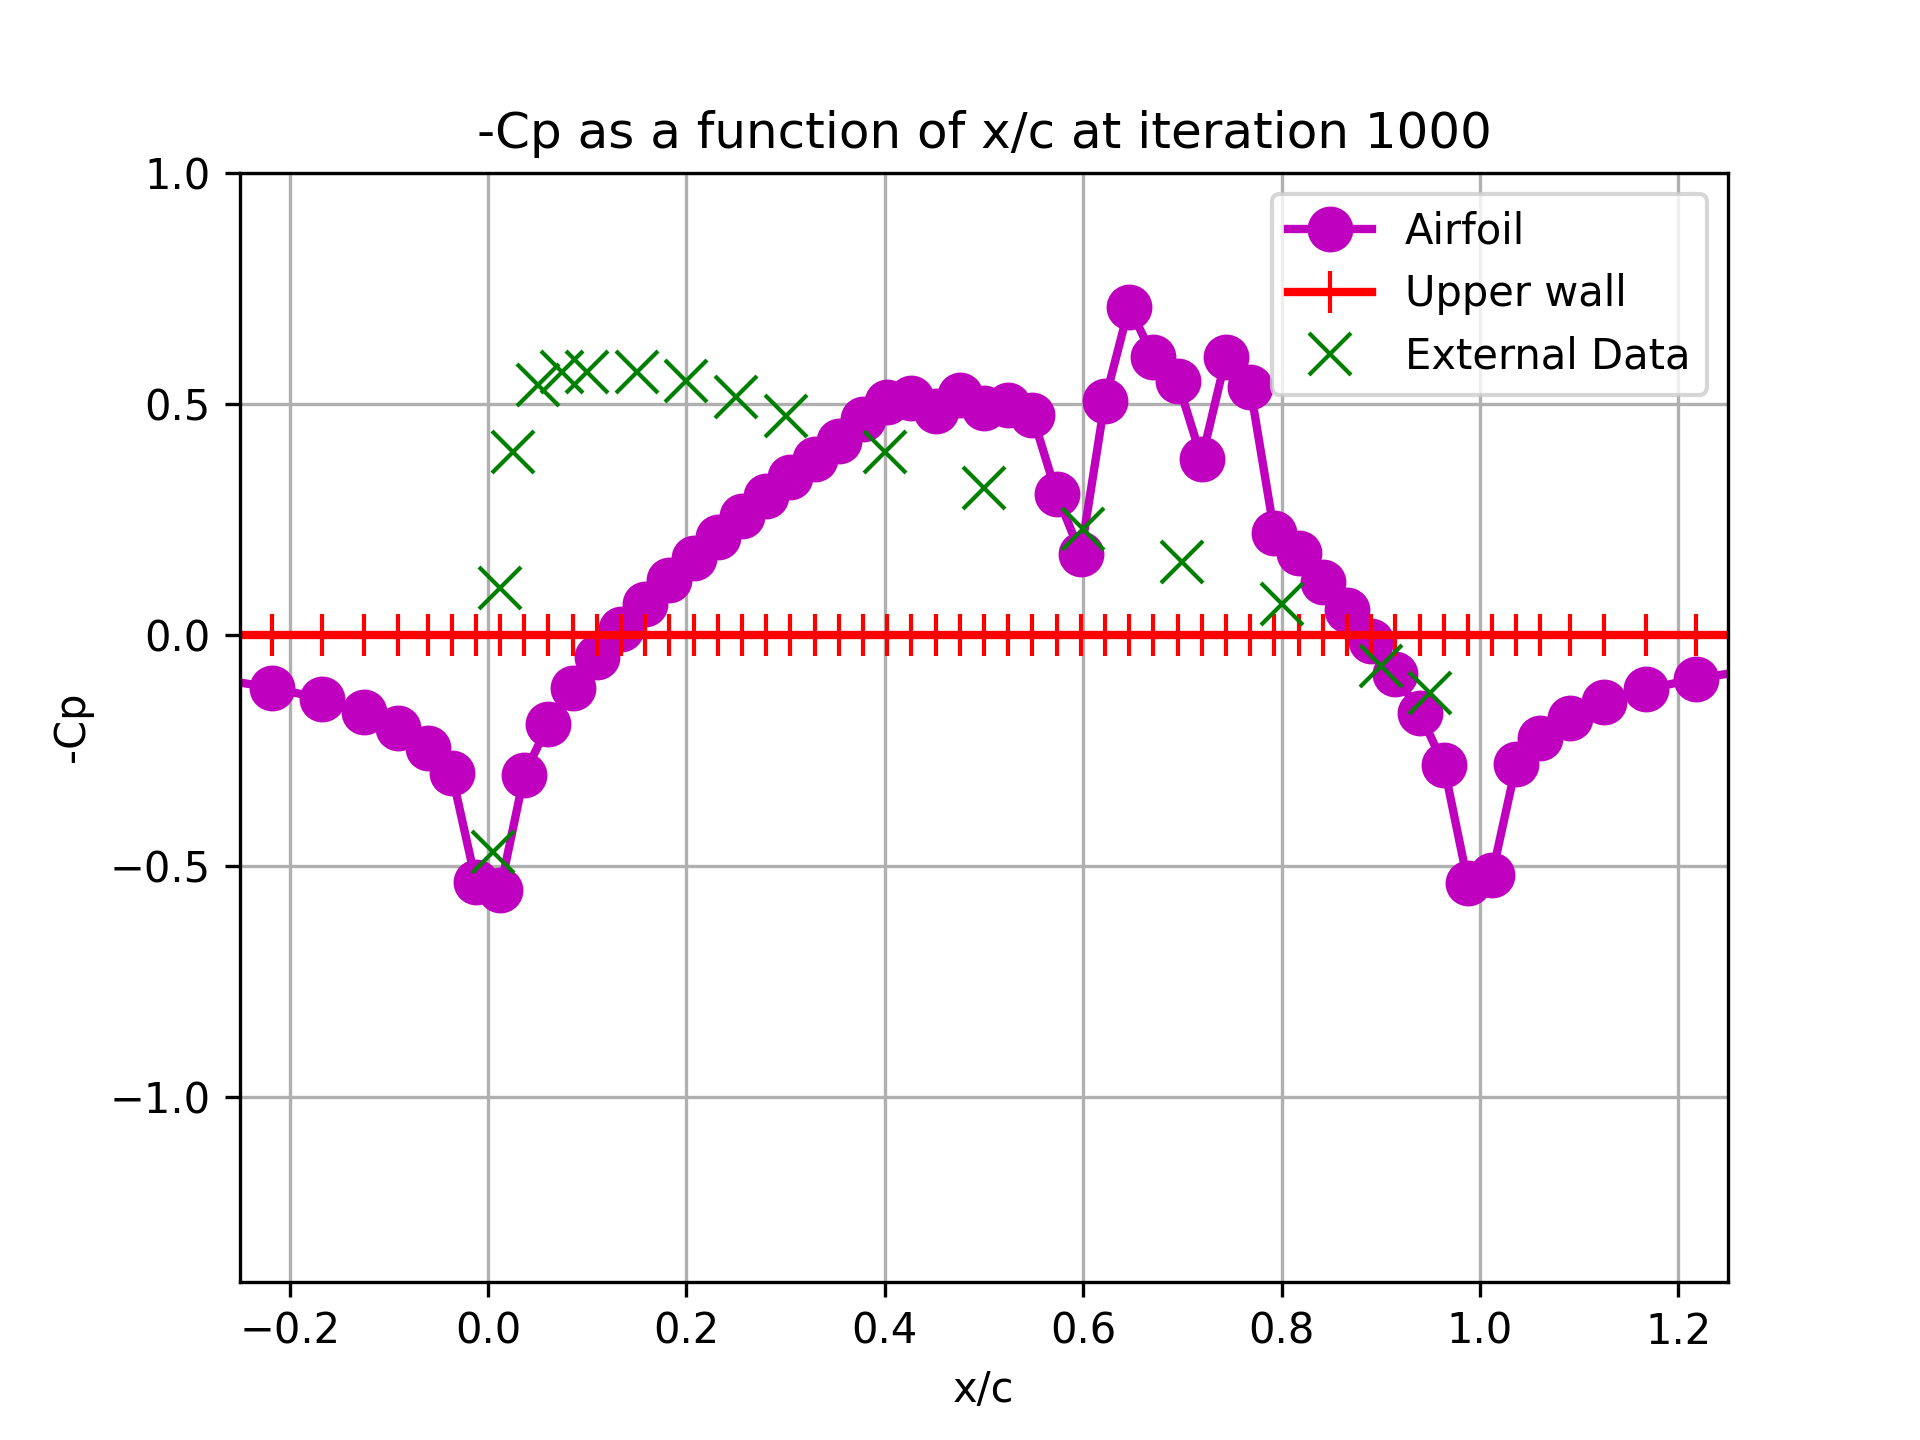
\includegraphics[width=0.75\textwidth,height=\textwidth,keepaspectratio]{images/pressure_coefficient-5.png}
    \caption{Pressure distribution $-C_p$ compared to $x/c$ along the airfoil surface for Biconvex 0010 airfoil at $M_\infty = 0.80$.}
    \label{fig:pressure_coefficient-5}
\end{figure}

\begin{figure}
    \centering
    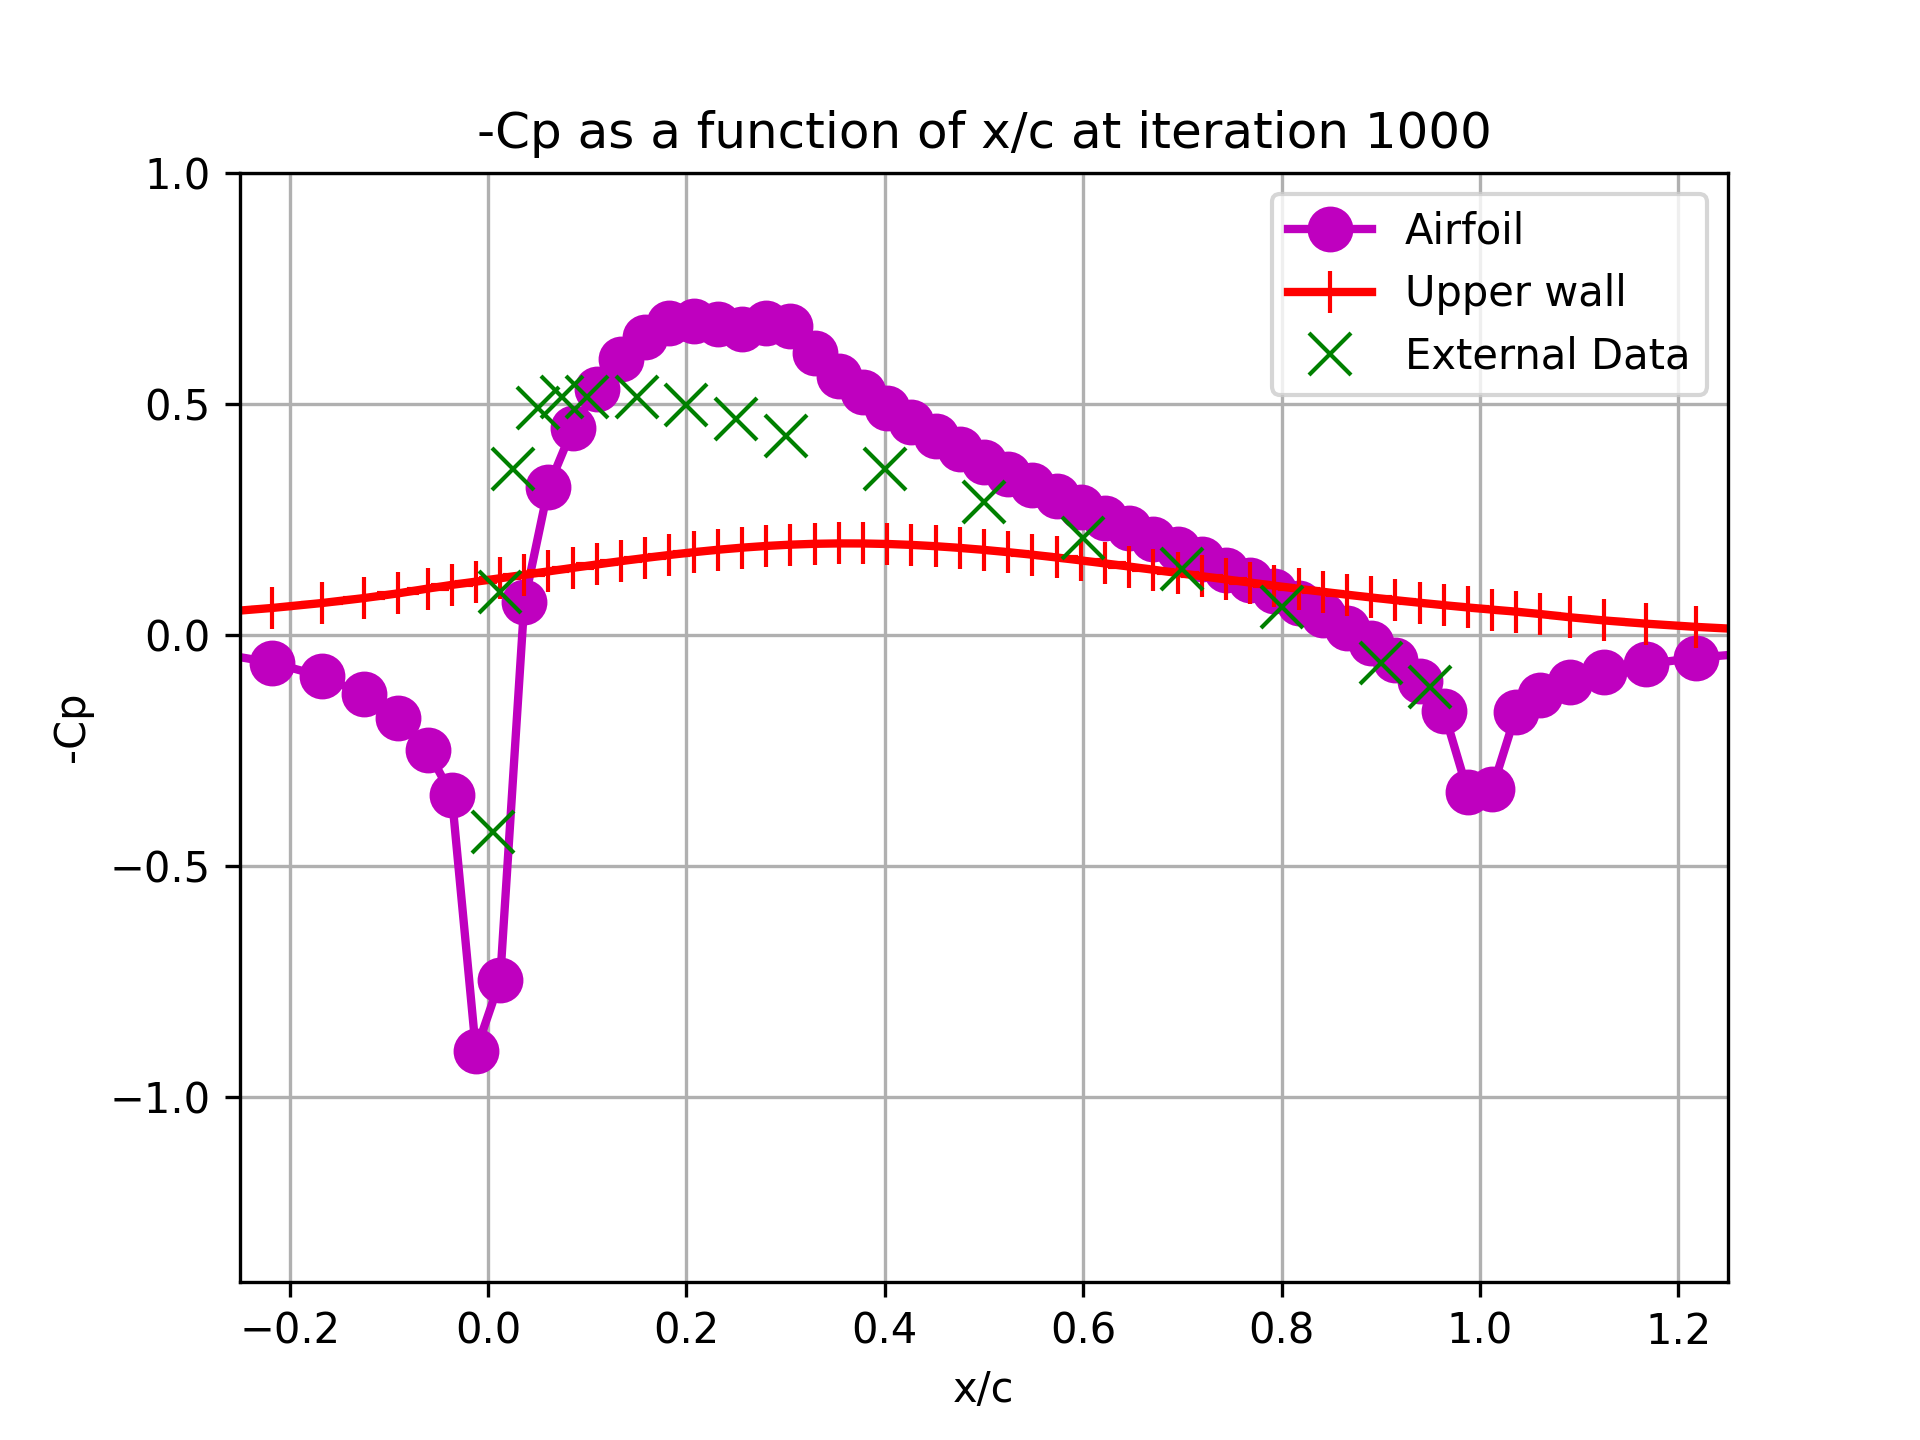
\includegraphics[width=0.75\textwidth,height=\textwidth,keepaspectratio]{images/pressure_coefficient-6.png}
    \caption{Pressure distribution $-C_p$ compared to $x/c$ along the airfoil surface for NACA 0010 airfoil at $M_\infty = 0.75$ with a wind tunnel.}
    \label{fig:pressure_coefficient-6}
\end{figure}

\begin{figure}
    \centering
    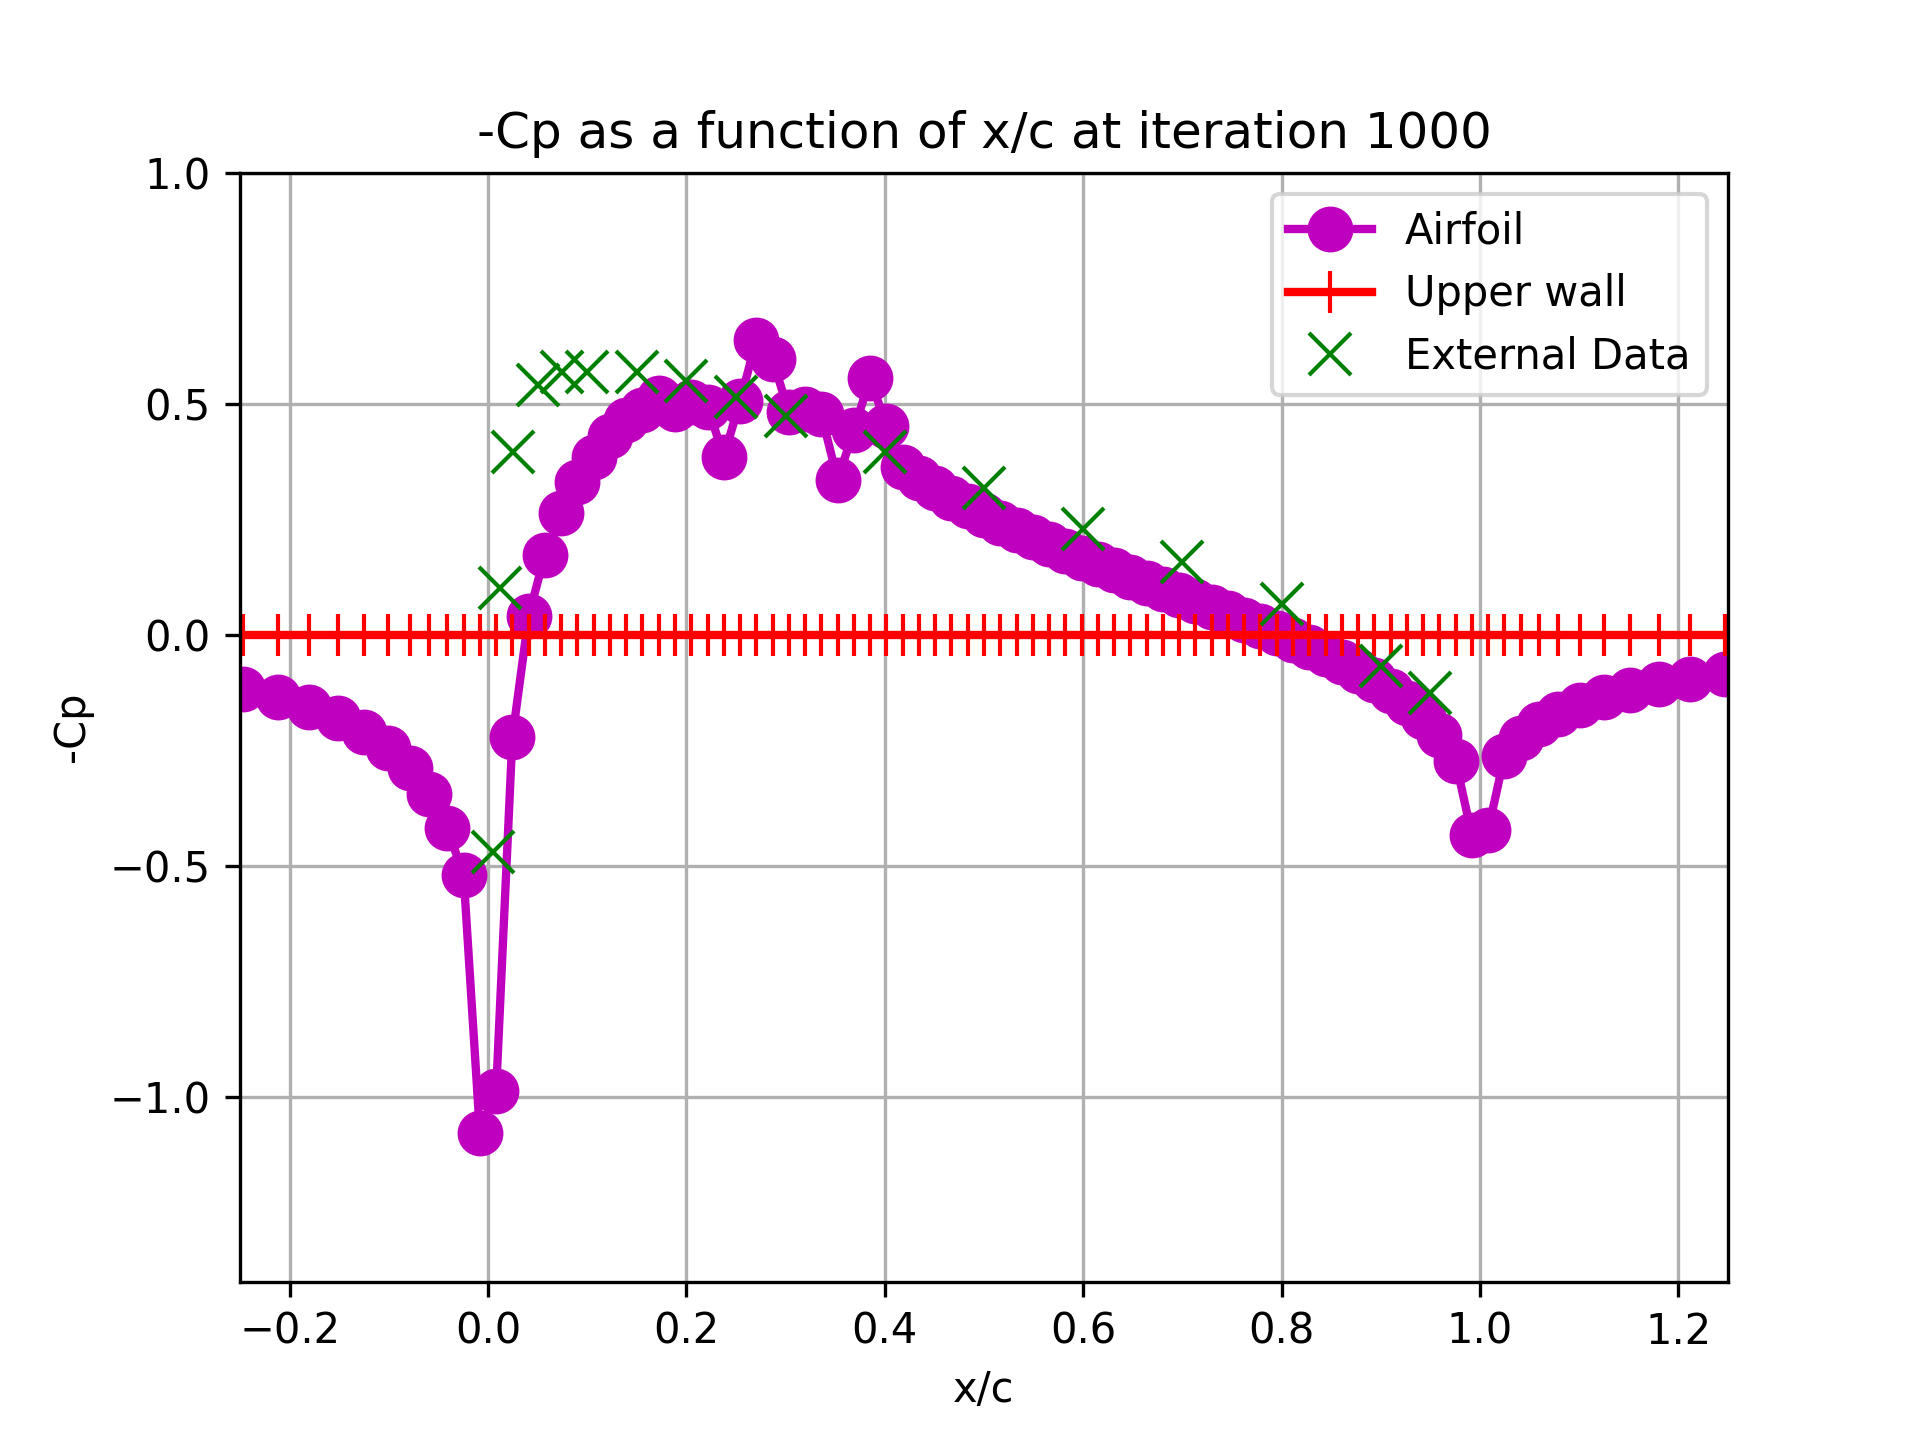
\includegraphics[width=0.75\textwidth,height=\textwidth,keepaspectratio]{images/pressure_coefficient-7.png}
    \caption{Pressure distribution $-C_p$ compared to $x/c$ along the airfoil surface for NACA 0010 airfoil at $M_\infty = 0.80$ using a stretched mesh.}
    \label{fig:pressure_coefficient-7}
\end{figure}

\vspace{1cm}


\noindent {\bf Try to verify the pressure distribution by independent means. Plot the representative convergence histories showing the log10 of the L2 norm of the residual versus iteration number. }\\

We can plot the $log_{10}$ of the $L^2$ norm of the residual versus the iteration number for cases 1-6 as shown in Figure \ref{fig:residual_history-7.png}.

\begin{figure}
    \centering
    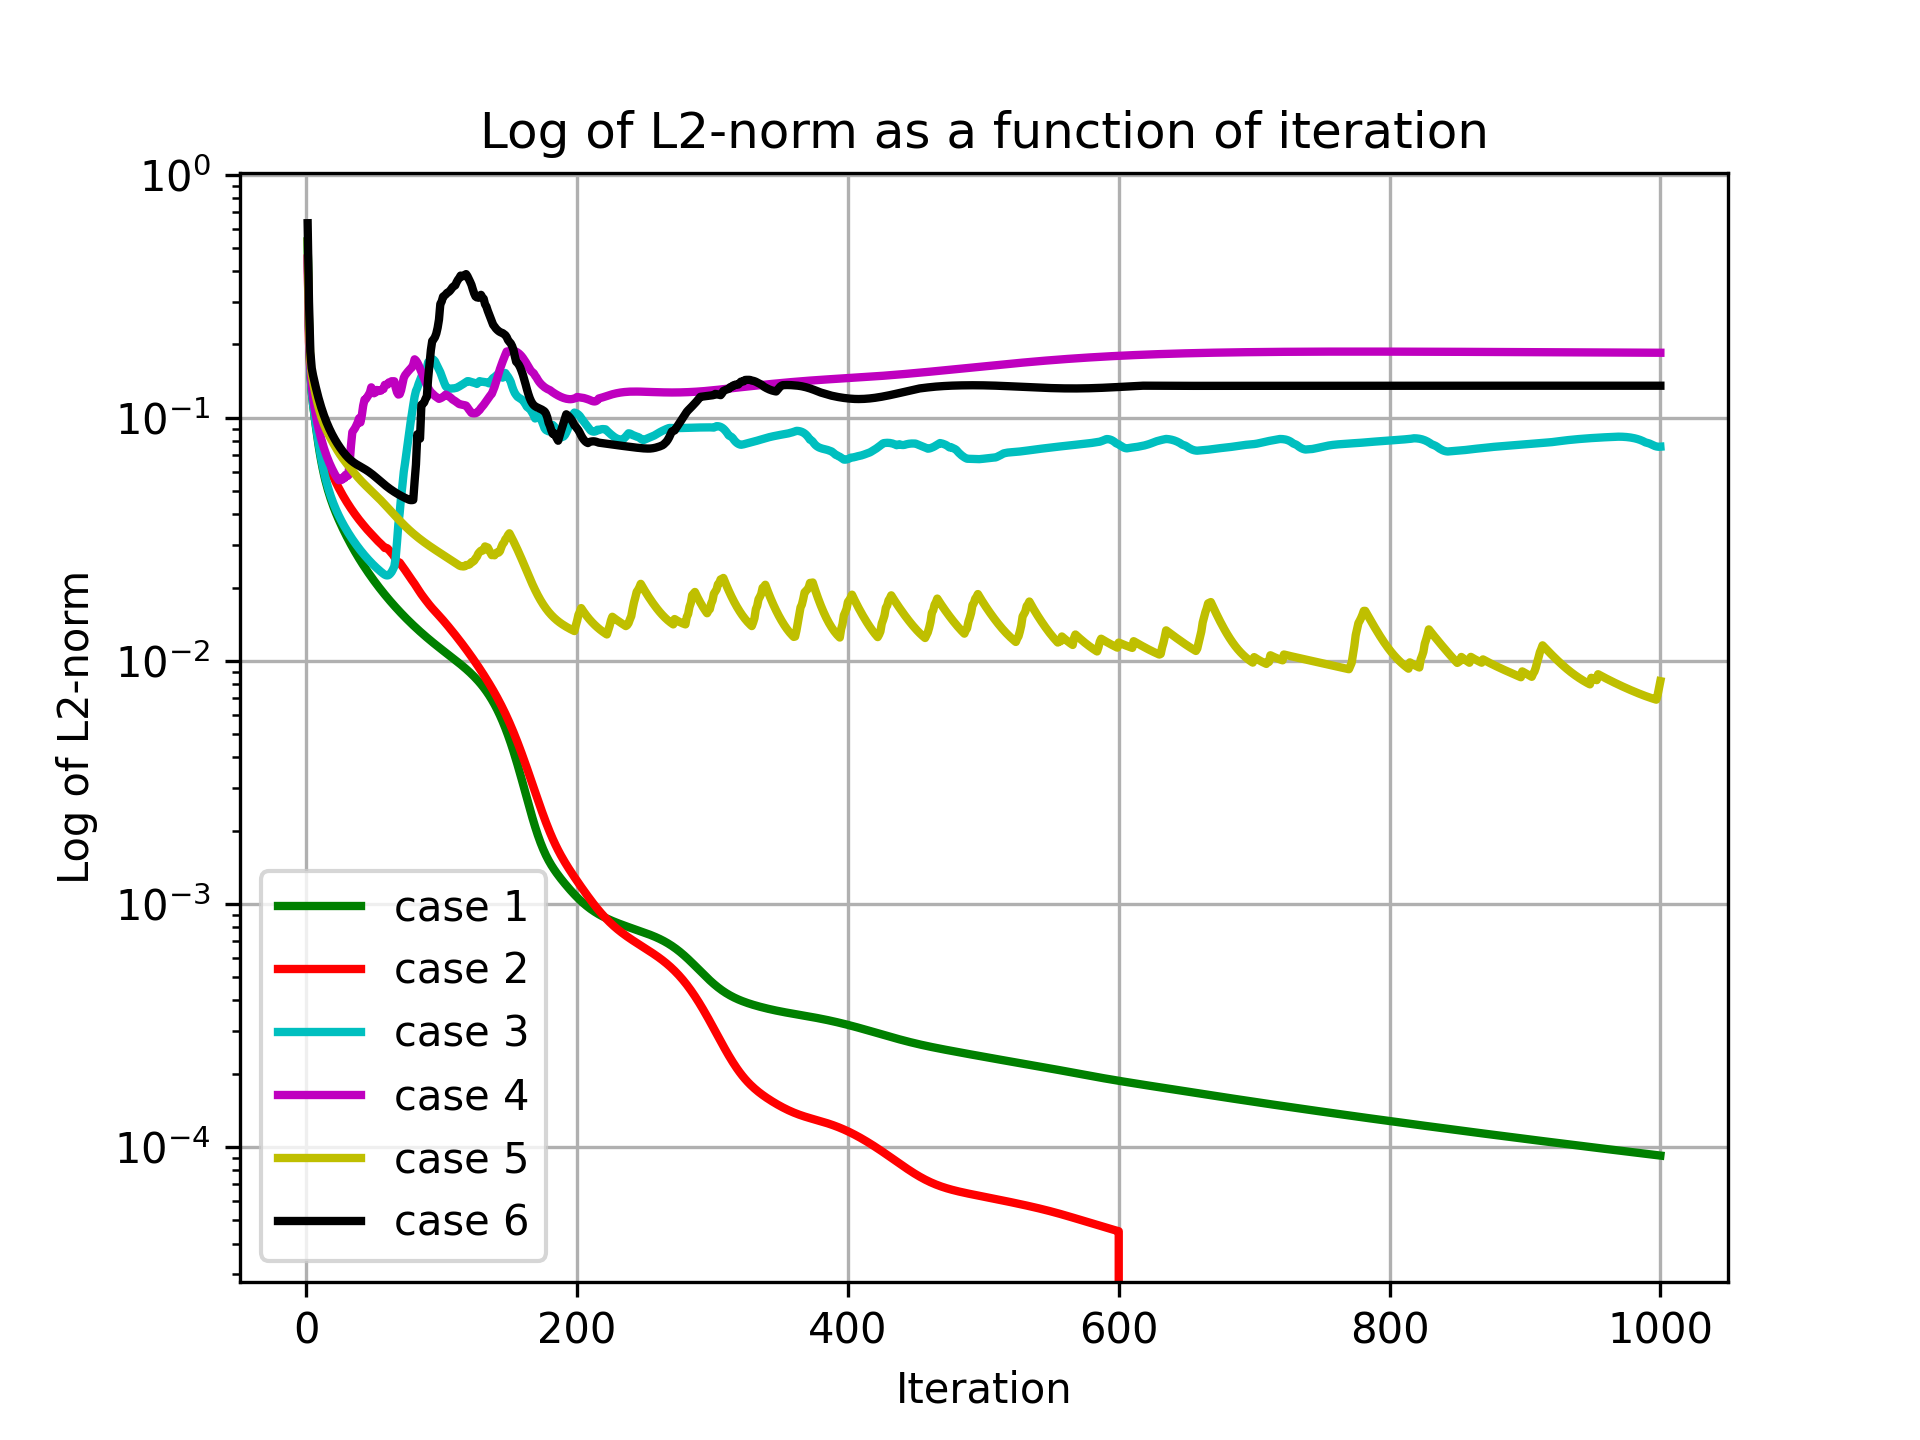
\includegraphics[width=0.75\textwidth,height=\textwidth,keepaspectratio]{images/residual_history-7.png}
    \caption{Convergence history of the six cases presented in Table \ref{tab:results}.}
    \label{fig:residual_history-7.png}
\end{figure}


\vspace{1cm}




\noindent {\bf Include a plot for the transonic cases with $M_\infty = 0.80$ showing the number of supersonic points (A$<$0) versus iteration number.}\\

Looking at case 4, we can plot the number of supersonic points per iteration number as shown in Figure \ref{fig:supersonic_points-4}

\begin{figure}
    \centering
    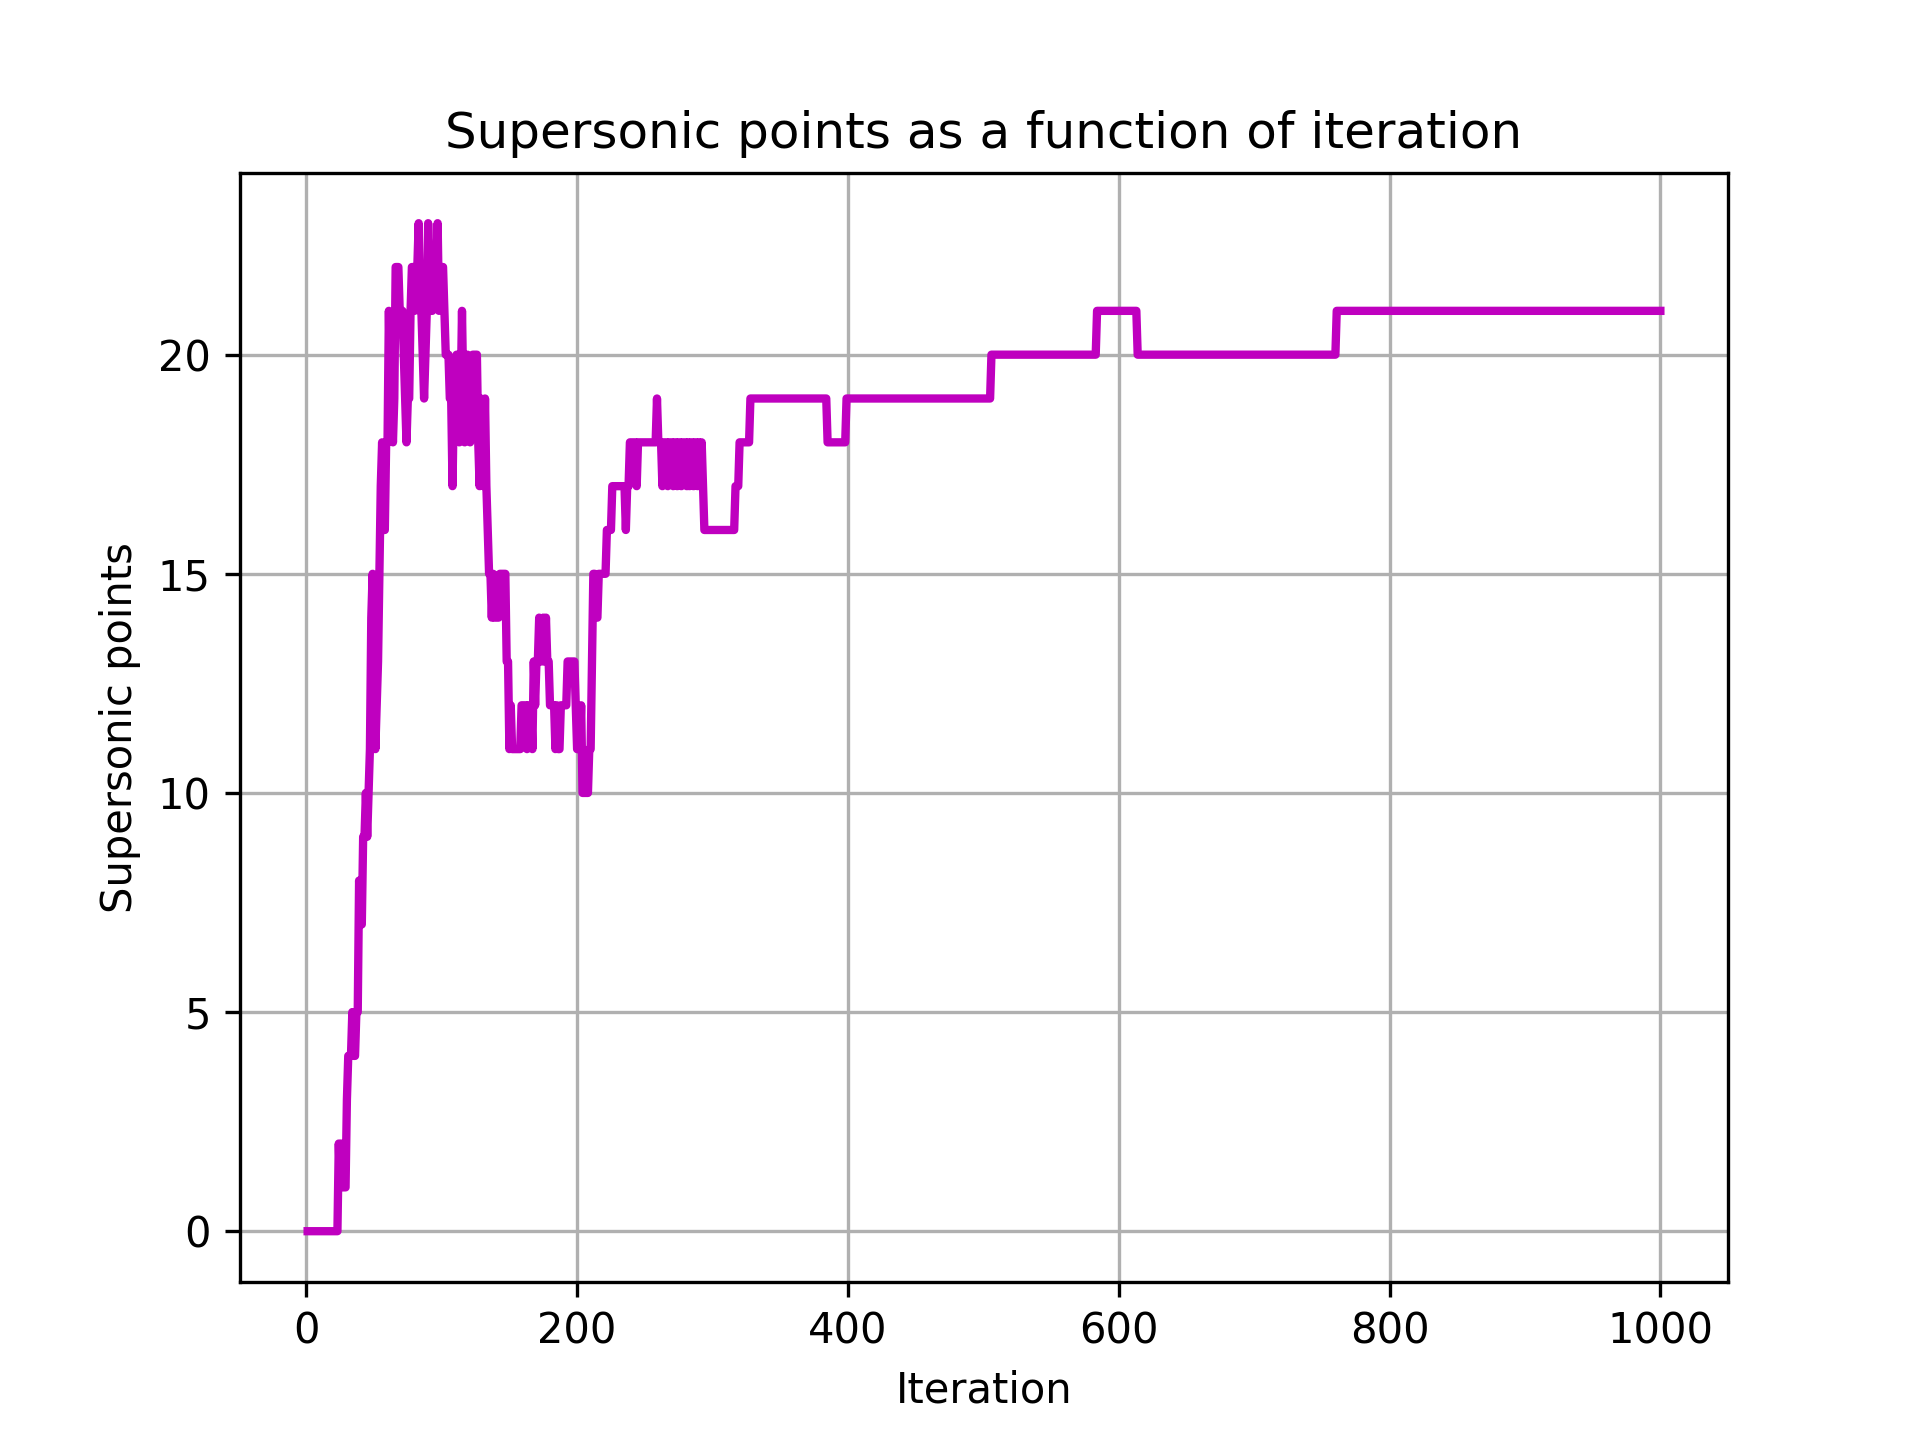
\includegraphics[width=0.75\textwidth,height=\textwidth,keepaspectratio]{images/supersonic_points-5.png}
    \caption{Number of supersonic points per iteration for a Biconvex airfoil with $M_\infty = 0.80$}
    \label{fig:supersonic_points-4}
\end{figure}

\vspace{1cm}




\noindent {\bf Note any observations and/or problems encountered. Cite any discrepancies and attempt to explain them. Are the convergence results what you expected? }\\

Looking at the pressure coefficient for cases 1-6 shown in Figures \ref{fig:pressure_coefficient-2} - \ref{fig:pressure_coefficient-7} respectively, 

\vspace{1cm}



\noindent {\bf Plot either the velocity vector field or streamlines for one of the transonic cases, as well as contours of the potential function, pressure, and/or Mach number (you can set the limits to: $-0.5 < x < 1.5$ and $0 < y <2$).}\\

Looking at case 4, we can plot the contours of the pressure shown in Figure \ref{fig:cp_contours-5} and the streamlines shown in Figure \ref{fig:velocity_vectors-5}.

\begin{figure}
    \centering
    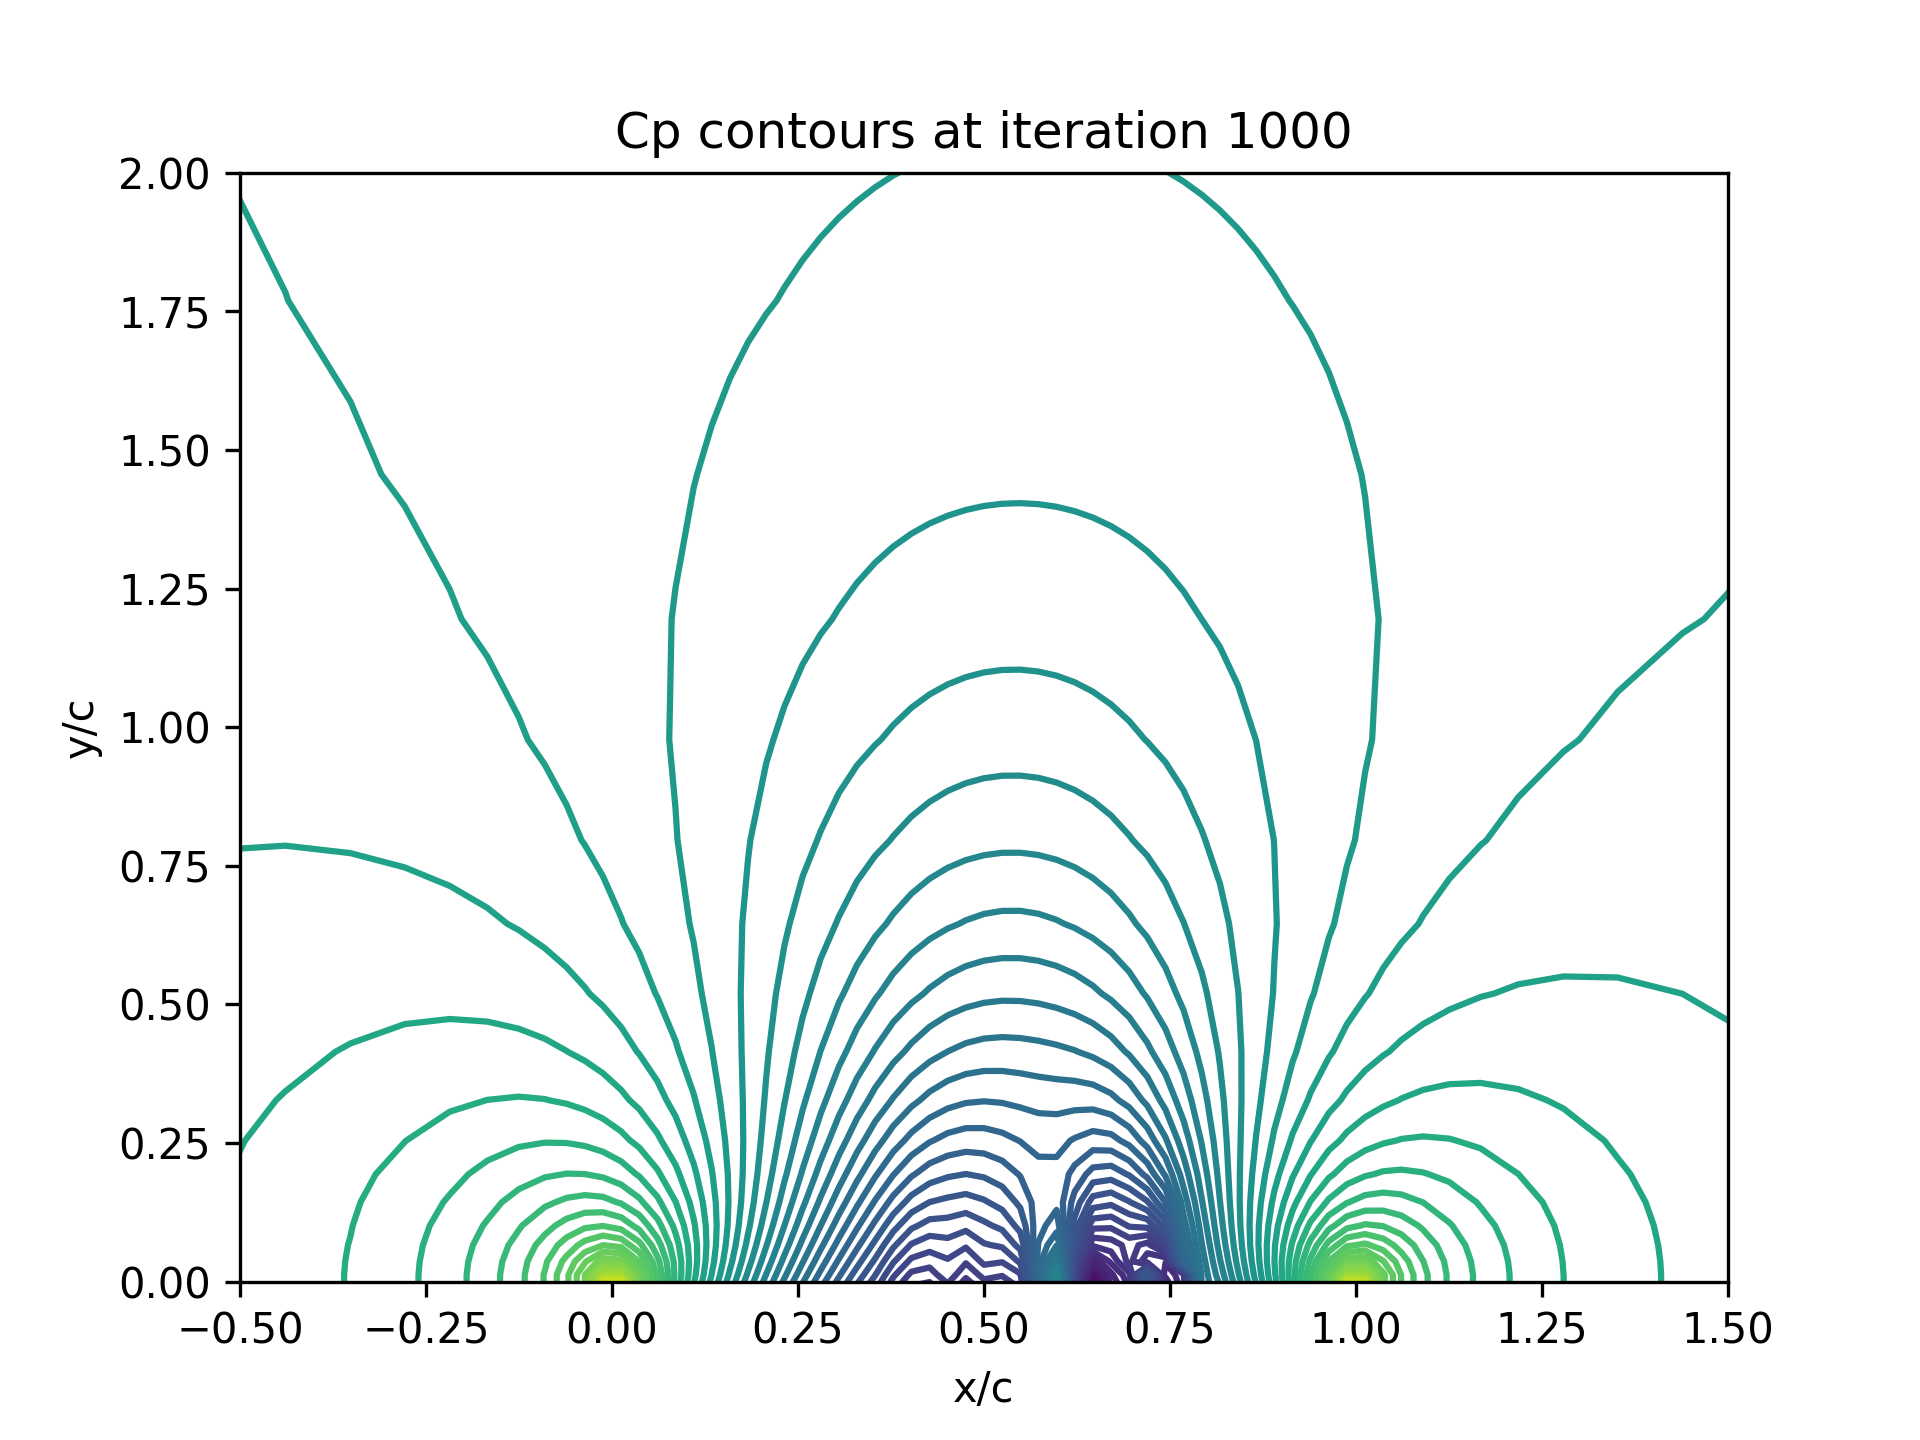
\includegraphics[width=0.75\textwidth,height=\textwidth,keepaspectratio]{images/cp_contours-5.png}
    \caption{Contour plot of $-C_p$ from $-0.5 < x < 1.5$ and $0 < y <2$ with a Biconvex airfoil with $M_\infty = 0.80$}
    \label{fig:cp_contours-5}
\end{figure}

\begin{figure}
    \centering
    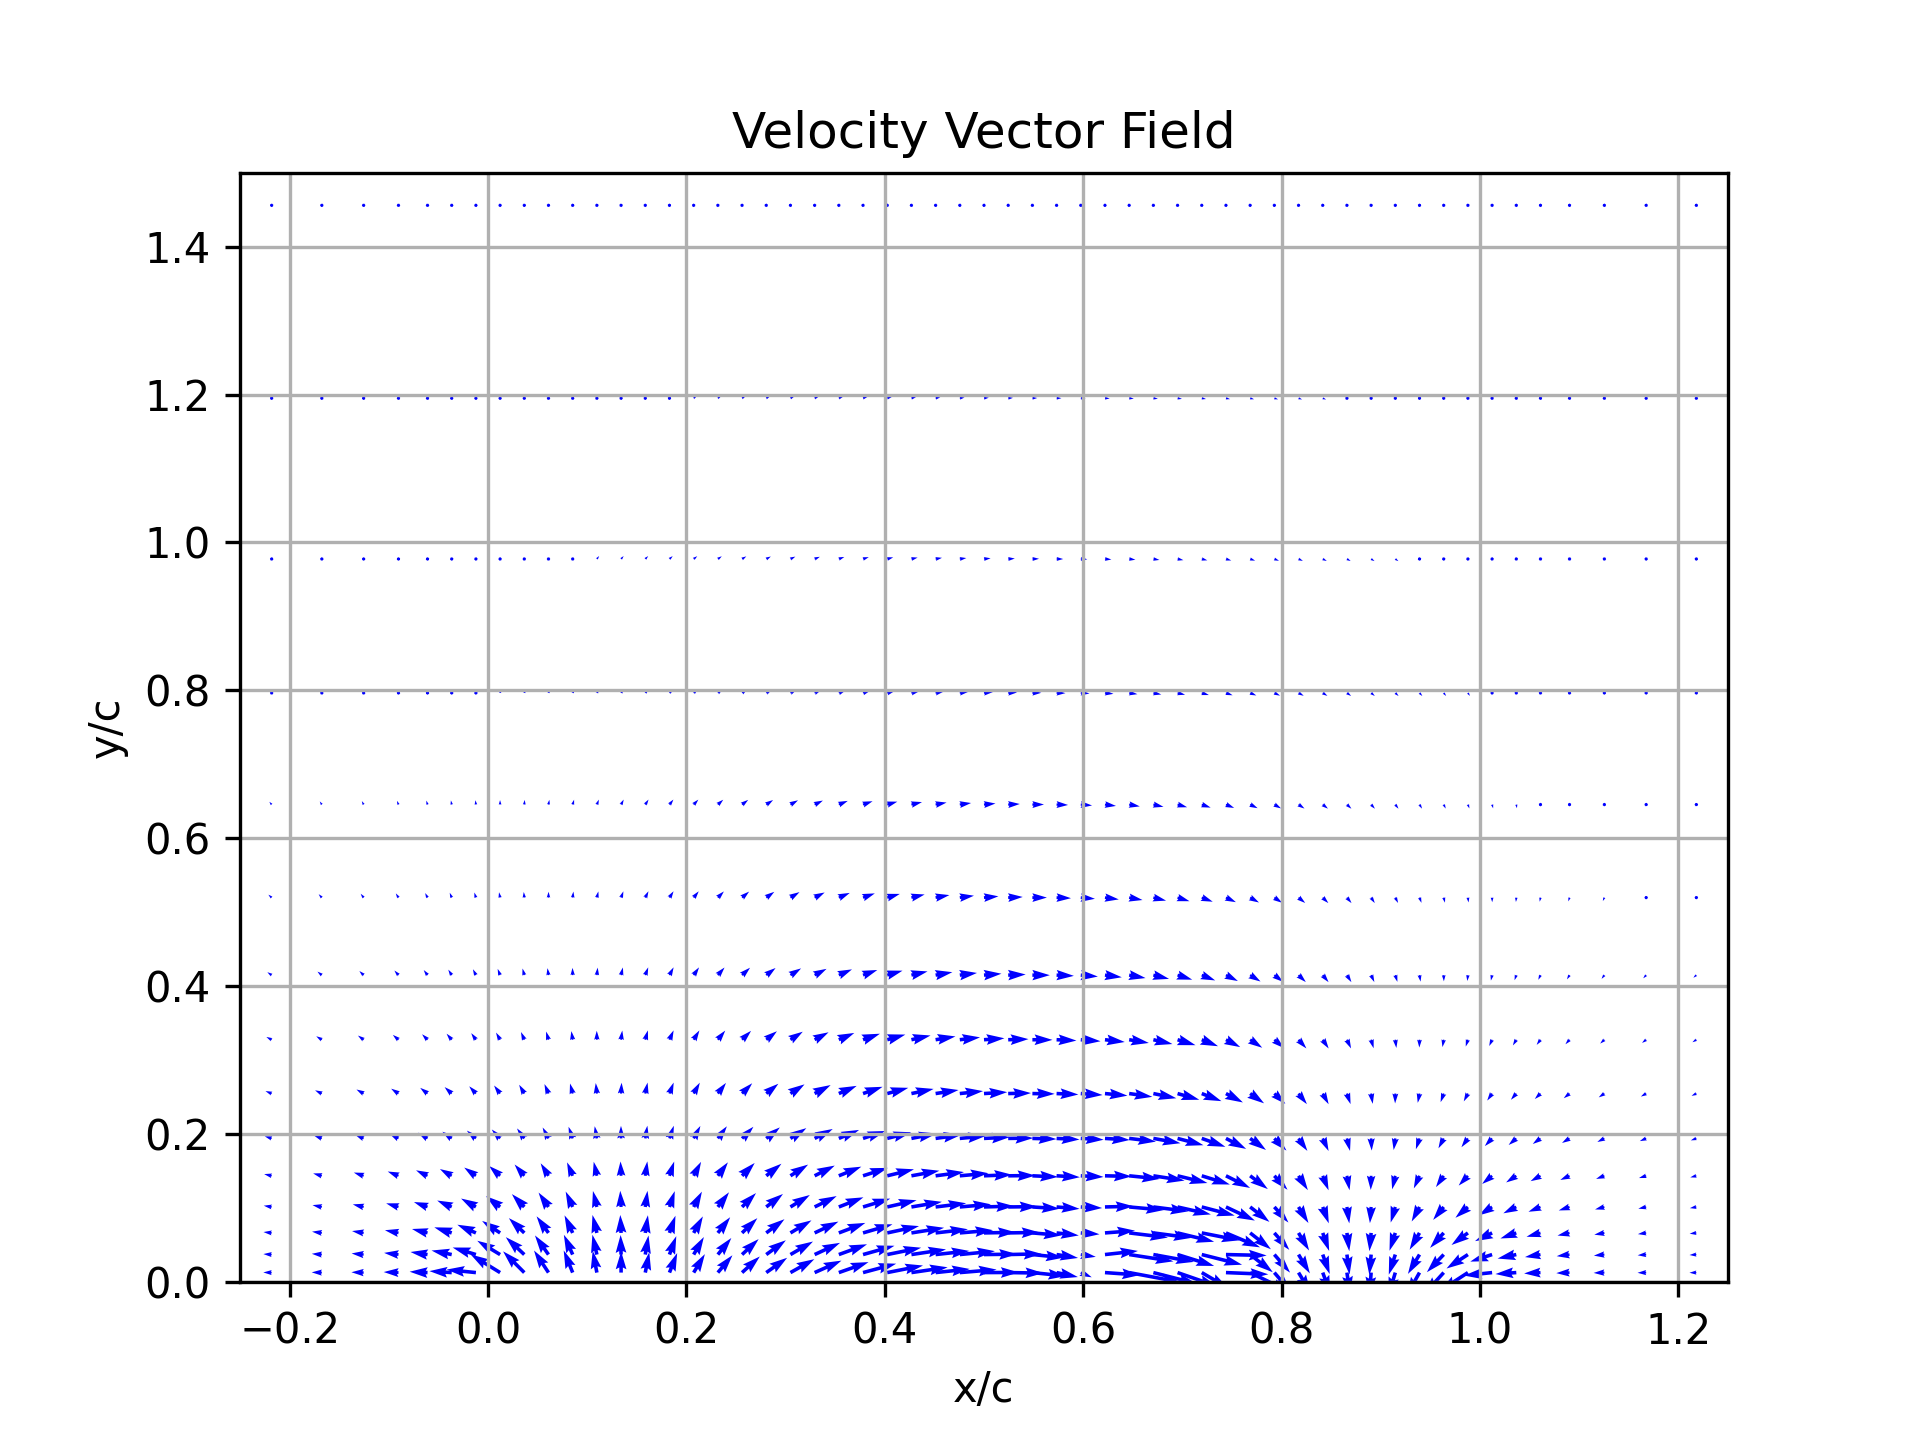
\includegraphics[width=0.75\textwidth,height=\textwidth,keepaspectratio]{images/velocity_vectors-5.png}
    \caption{Streamlines from $-0.5 < x < 1.5$ and $0 < y <2$ with a Biconvex airfoil with $M_\infty = 0.80$}
    \label{fig:velocity_vectors-5}
\end{figure}